\subsection{Module Federation}\label{subsection:background:micro-frontend:module-federation}

Webpack 5 introduced a new native plugin called Module Federation. Module Federation allows chunks of \ac{JS} code to be loaded synchronously or asynchronously during runtime, allowing multiple teams to work in isolation and take care of the application composition. Lazy-loading different \ac{JS} chunks take place behind the scenes. \cite[81]{book:2021:mezzalira:applied-methods:building-micro-frontends}

\bigskip

\noindent Typically a module-federation application consists of two parts: \cite[81]{book:2021:mezzalira:applied-methods:building-micro-frontends}

\begin{itemize}
  \item The \texttt{host}, which is the main application is therefore responsible for loading the remote micro-frontends or libraries.
  \item The \texttt{remote}, which is either a micro-frontend or library, is consumed by the host. A remote can expose multiple modules that can be lazy-loaded inside the application.
\end{itemize}

\noindent Exposing micro-frontends or libraries with Module Federation is very simple, and developers can import the remote micro-frontends and compose the view as they would with normal modules. Another essential feature of Module Federation for micro-frontend architectures is the possibility of sharing the same instance of external dependencies across all micro-frontends. If a library should be shared across multiple micro-frontends, Module Federation will make sure to load only one instance. For example, if all micro-frontends should use version 15 of Angular, the version of the shared dependency has to be specified in the Module Federation configuration. At run time, Webpack will load only one version of Angular for all micro-frontends that use it. Working with different versions of the same library is also possible, and Module Federation will put each version in a different scope to avoid clashes at runtime. Module Federation is not just limited to the client but is also viable if the application is rendered on the server. \cite[82-83]{book:2021:mezzalira:applied-methods:building-micro-frontends}

\subsubsection{Performance}\label{subsubsection:background:micro-frontend:module-federation:performance}

Image multiple teams working on the same application. Each team develops one or more micro-frontend, and the teams have agreed to use the same \ac{UI} component libraries for the micro-frontend architecture. These libraries can be automatically shared with Module Federation, and they will be loaded only once at the beginning of the project, therefore all projects have the same version of the \ac{UI} components. Using only one instance of a dependency for multiple applications saves the browser from downloading a large \ac{JS} bundle. Module Federation can also load new micro-frontends during runtime, instead of defining them all in the configuration. \cite[83]{book:2021:mezzalira:applied-methods:building-micro-frontends}

\subsubsection{Composition}\label{subsubsection:background:micro-frontend:module-federation:composition}

Using Module Federation is as easy as importing external \ac{JS} chunks lazy-loaded inside a project. Lazy loading describes a technique, that defers the loading of resources until they are needed. The technique is especially important in web development to reduce the time until a page is rendered initially. Resources like images are loaded only when they are visible on the screen. The composition of applications occurs on the client side at runtime, when an application shell is used for loading different micro-frontends, or on the server when a server-side rendered application is used. \cite[84]{book:2021:mezzalira:applied-methods:building-micro-frontends}

\subsubsection{Shared code}\label{subsubsection:background:micro-frontend:module-federation:shared-code}

Module Federation makes sharing code between multiple teams very easy. Module federation allows sharing code between multiple micro-frontends bidirectional. This Webpack plugin flattens the hierarchy between the application shell and the remote micro-frontends. But sharing code from micro-frontends to the container application is discouraged because a unidirectional implementation brings several advantages such as the following: \cite[84]{book:2021:mezzalira:applied-methods:building-micro-frontends}

\begin{itemize}
  \item The code is easier to debug, as the location of the code is known.
  \item It is less prone to errors, and the code communicates in controllable ways.
  \item It is more efficient, as the micro-frontend knows the boundaries of each part of the application.
\end{itemize}

\subsubsection{Module Federation 101}\label{subsubsection:background:micro-frontend:module-federation:101}

Module Federation allows a \ac{JS} application to dynamically load and run code from another bundle. Module Federation provides two key concepts that are very important before working with it. \cite[118-119]{book:2021:mezzalira:applied-methods:building-micro-frontends}

\begin{itemize}
    \item \texttt{Host}: The host is the that container loads the shared libraries and micro-frontends at runtime.
    \item \texttt{Remote}: The bundle that should be consumed by the host.
\end{itemize}

\noindent Figure \ref{fig:background:micro-frontend:module-federation:module-federation-architecture} shows a host application that loads multiple remotes. The host is also called application shell, whereas a remote is a micro-frontend.

\ifshowImages
\begin{figure}[H]
  \centering
  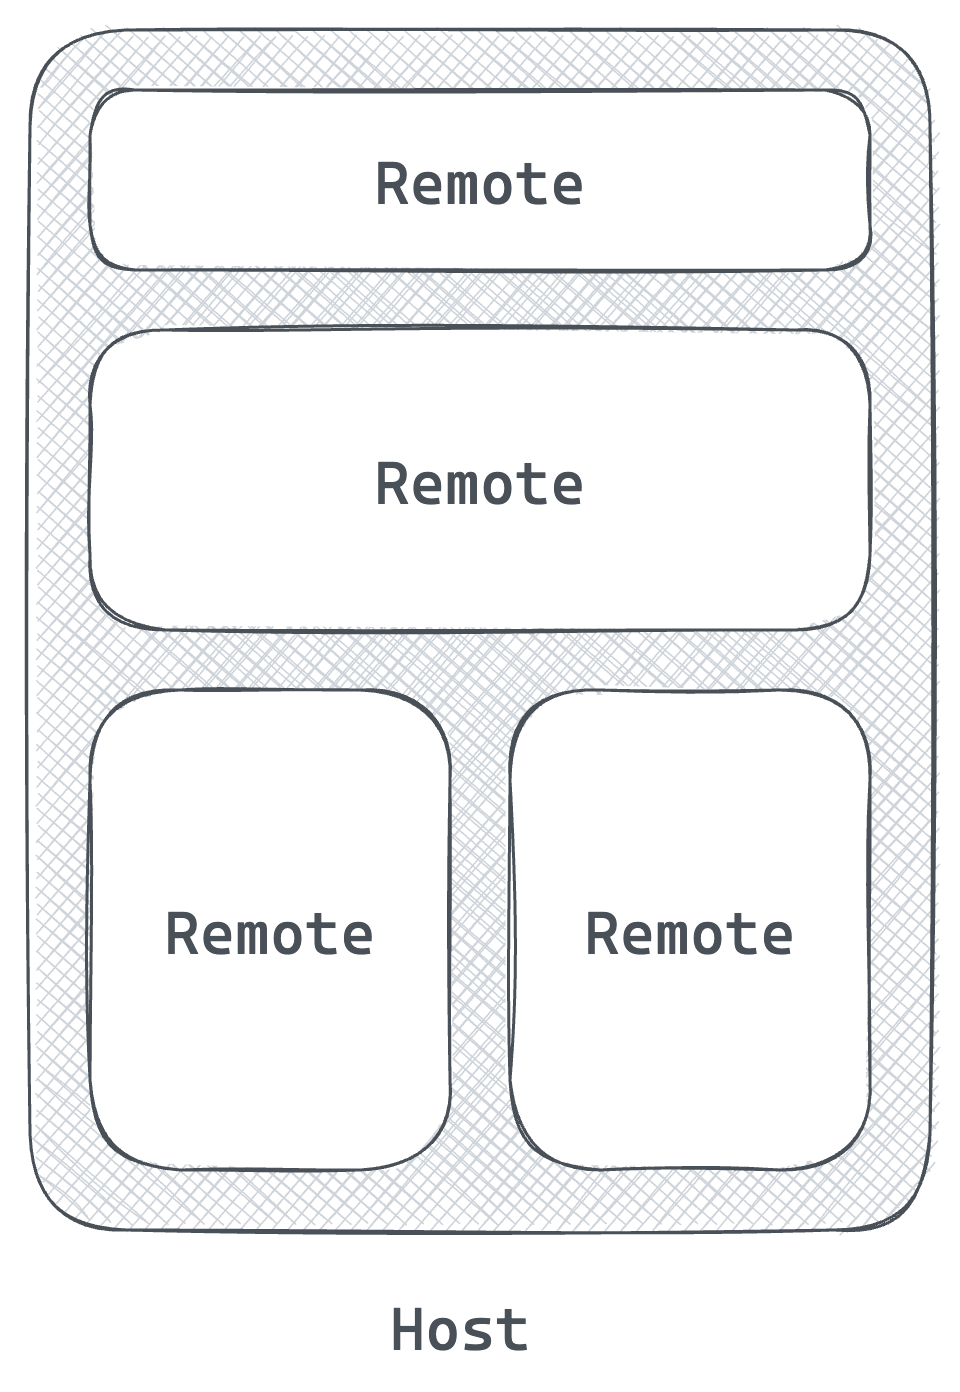
\includegraphics[width=0.25\linewidth]{images/background/micro-frontends/module-federation/module-federation-architecture.png}
  \caption{A micro-frontend architecture with an application shell and multiple remotes. (Adapted from \cite[119]{book:2021:mezzalira:applied-methods:building-micro-frontends})}\label{fig:background:micro-frontend:module-federation:module-federation-architecture}
\end{figure}
\fi

\noindent Module Federation allows the code to be shared bidirectional, allowing a remote to share the whole bundle with a application shell and vice versa. However, bidirectional sharing can complicate the architecture quite easily. The best approach is to share only in one direction, so the application shell never shares code with the remote. \cite[119]{book:2021:mezzalira:applied-methods:building-micro-frontends}

\subsubsection{Configuring Module Federation}\label{subsubsection:background:micro-frontend:module-federation:configuring-module-federation}

Configuring module federation is done inside Webpack's configuration file. Listing \ref{fig:background:micro-frontend:module-federation:configuring-module-federation} shows the configuration of the application shell application.

\ifshowListings
\begin{listing}[H]
  \begin{minted}{typescript}
plugins: [
  new ModuleFederationPlugin({
    name: 'Host',
    remotes: {
      Contact: 'Contact@http://localhost:4201/remoteEntry.js',
      Sales: 'Sales@http://localhost:4202/remoteEntry.js',
      ...
    },
    shared: [
      '@angular/core': { singleton: true },
      '@angular/router': { singleton: true },
      '@angular/material': { singleton: true },
      ...
    ]
  })
]
  \end{minted}
  \caption{Configuring Module Federation for the application shell.}\label{fig:background:micro-frontend:module-federation:configuring-module-federation}
\end{listing}
\fi

\noindent First, the \texttt{name} of the application has to be defined, in this case, \texttt{Host}. The \texttt{remotes}-object specifies the modules that should be consumable by the application shell. Every remote consists of an ID and an associated \ac{URL} and the \texttt{remoteEntry.js} contains a map of all \ac{JS} chunks for the micro-frontend that should be fetched. These two values are separated through an \texttt{@} symbol. \cite[124]{book:2021:mezzalira:applied-methods:building-micro-frontends}

\bigskip

\noindent For example, the contact micro-frontend has the ID \texttt{Contact} and the \ac{URL} \texttt{http:\slash \slash localhost:4201\slash remoteEntry.js}. If the application shell loads the contact micro-frontend, Module Federation will fetch the \texttt{remoteEntry.js} file to understand which \ac{JS} chunks should be loaded and which dependencies should be shared between all micro-frontends. \cite[125]{book:2021:mezzalira:applied-methods:building-micro-frontends}

\bigskip

\noindent The \texttt{expose} option can be used to define the functionality that should be consumable by other applications using Module Federation. The \texttt{shared} array contains the libraries, which should be shared across all micro-frontends. Module Federation requires specifying the dependencies to be shared with the remote and the application shell. This can be all the dependencies of the micro-frontend and the application shell. Then Webpack and Module Federation will create multiple \ac{JS} files containing the dependencies, downloading them only once for the user's session across all micro-frontends. \cite[125]{book:2021:mezzalira:applied-methods:building-micro-frontends}

\bigskip

\noindent As shown inside the \texttt{shared}-array in Listing \ref{fig:background:micro-frontend:module-federation:configuring-module-federation}, a part of the libraries that should be shared is listed. How the dependencies are shared can be configured in many ways. The property \texttt{singleton} specifies that a library can be only loaded once. The dependencies that are exposed through Module Federation can be loaded synchronously or asynchronously through the \texttt{eager} property. It is recommended to load the dependencies asynchronously, as the application can be loaded faster. With \texttt{requiredVersion} the required version of the library can be configured. The option \texttt{strictVersion} is used to specify that the exact version which is specified should be loaded. If the version is different, Module Federation throws an error. These are only some of the configuration properties available, and many more exist. \cite[125]{book:2021:mezzalira:applied-methods:building-micro-frontends}
